\begin{frame}
\titlepage % Print the title page as the first slide
\end{frame}
\begin{frame}
\frametitle{Physical Unclonable Functions 101}
\begin{itemize}
\item	Silicon fingerprint via challenge-response pair (CRP)
	\begin{itemize}
	\item	Entropy from process variation
	\item	Invisible when power off and secure against physical attacks
	\item	Secure key generation and device authentication
	\end{itemize}
\item	Strong PUFs provide a much larger CRP space than Weak PUFs 
\begin{figure}
\centering
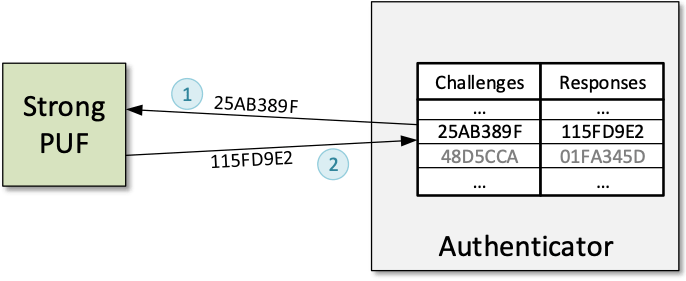
\includegraphics[width=.8\linewidth]{fig/PUFCRP.png}
\end{figure}
    \begin{itemize}
        \item Weak PUFs: SRAM PUF, Butterfly PUF
        \item Strong PUFs: Arbiter PUF, Ring-Oscillator (RO) PUF, controlled PUF
    \end{itemize}
\end{itemize}
\end{frame}

\begin{frame}
\frametitle{Machine Learning Attacks on Strong PUFs}
\begin{itemize}
    \item CRPs can be modelled by function $r=f(\mathbf{c})$
        \begin{itemize}
            \item Linear model: Arbiter PUF, RO PUF
            \item Non-linear model: XOR Arbiter PUF, SCA PUF
        \end{itemize}
    \item TODO: put a figure of ml attack flow
    \item Flow of ML attacks:
        \begin{itemize}
            \item Collect a bunch of CRPs for given PUF 
            \item Train a mathematical model $r = f'(\mathbf{c})$
            \item Use $f'$ to fake $f$
        \end{itemize}
\end{itemize}
\end{frame}

\begin{frame}{Problem: Can We Engineer a ML Resistant PUF?}
\begin{itemize}
    \item Arbiter PUF successfully attacked by support vector machine (SVM)
    \item Arbiter PUF variants by strengthening non-linearity successfully attacked by advanced ML attacks:
        \begin{itemize}
            \item Bi-stable Ring PUF, Feed-forward PUF, Lightweight secure PUF attacked by
            \item Interpose-PUF, XOR Arbiter PUF attacked by deep learning
        \end{itemize}
    \item Empirically-demonstrated ML resistance for PUFs with intrinsic nonlinearity 
    \item ML resistance via established cryptographic primitives
        \begin{itemize}
            \item Controlled PUF, AES PUF, computational fuzzy extractor
        \end{itemize}
\end{itemize}    
\end{frame}

\begin{frame}{Our Contribution}
\begin{itemize}
    \item A strong PUF with provable ML resilience derived from lattice cryptography.
    \item Efficient hardware implementation via distributional relaxation
\end{itemize}    
\end{frame}

\begin{frame}{Formal Definition of ML Resistance}
\begin{itemize}
    \item Intuitively, good measure of ML hardness need:
        \begin{itemize}
            \item Easy to learn: a learning algorithm can find a model with good quality, using a small number of CRPs, in a short time
            \item Hard to learn: \textbf{all possible learning algorithms fail, or they require a large number of CRPs, or a long running time}
        \end{itemize}
    \item Probably approximately correct (PAC) model is the only known formal framework for provable notion of ML resistance
        \begin{itemize}
            \item Definition: strong PUF $\mathcal{F}$ is PAC-learnable if there exists a polynomial-time algorithm $\mathcal{A}$ such that $\forall \epsilon > 0$, $\forall \delta >0$, for any fixed CRP distribution $\mathcal{D}$, and $\forall f\in\mathcal{F}$, given a training set of size $m$, $\mathcal{A}$ produces a candidate model $h\in\mathcal{H}$ with probability of, at least, $1-\delta$ such that
\begin{equation*}
\Pr_{(\mathbf{c},r)\sim\mathcal{D}}[f(\mathbf{c})\neq h(\mathbf{c})] < \epsilon.
\end{equation*}
        \end{itemize}
    \item Definition: strong PUF $\mathcal{F}$ is ML-resistant if it is not PAC-learnable
    \item k-bit concrete hardness: if the current best ML attack requires $2^k$ CPU operations 
    \item Challenge: are there known PAC non-learnable functions?
\end{itemize} 
\end{frame}

\begin{frame}{Decryption Functions Are not PAC Learnable}
\begin{itemize}
    \item A typical public-key cryptosystem
    
\end{itemize}    
\end{frame}

\begin{frame}{Decryption Functions Are not PAC Learnable}
\begin{itemize}
    \item Chosen plaintext attacks    
    \item Security against chosen plaintext attacks
\end{itemize}    
\end{frame}

\begin{frame}{Decryption Functions Are not PAC Learnable}
\begin{itemize}
    \item CRP space: challenge $\leftrightarrow$ ciphertext, response $\leftrightarrow$ plaintext (0/1)
    \item A successful learning algorithm could help construct a successful chosen plaintext attack
    \begin{itemize}
        \item TODO: add a figure how to turn learning algorithm to chosen plaintext attack
    \end{itemize}
    \item Theorem: If a public-key cryptosystem is secure against chosen plaintext attacks, then its decryption functions are not PAC-learnable (under the ciphertext input distribution).
    \begin{itemize}
        \item Implementing a PUF using decryption function
        \item Which cryptosystem and decryption function to pick?
    \end{itemize}
\end{itemize}    
\end{frame}

\begin{frame}{Lattice Problems}
\begin{itemize}
    \item A lattice $\mathcal{L}(\mathbf{V})$ is a set of integral linear combinations of a given basis $\mathbf{V}=\{\mathbf{v}_1,\mathbf{v}_2,\ldots, \mathbf{v}_n\}$:
\begin{equation*}
\mathcal{L}(\mathbf{V}) = \{a_1\mathbf{v}_1 + a_2\mathbf{v}_2+\ldots a_n\mathbf{v}_n: \: \forall a_i \in \mathbb{Z}\}.
\end{equation*}
TODO: add a figure of 2D lattice
    \item Several lattice based problems are assumed to be intractable 
    \begin{itemize}
        \item (Approximate) shortest vector problem (SVP), Approximate SIVP
    \end{itemize}
\end{itemize}
\end{frame}

\begin{frame}{Learning-With-Errors (LWE) Problem}
\begin{itemize}
    \item LWE problem: distinguish $(\mathbf{a}_i,b_i)$'s from a uniform distribution
    \begin{align*}
        b_1 &= \innerprod{\mathbf{a}_1,\mathbf{s}} + e_1\\
        b_2 &= \innerprod{\mathbf{a}_2,\mathbf{s}} + e_2\\
        \ldots\\
        b_m &= \innerprod{\mathbf{a}_m,\mathbf{s}} + e_m
    \end{align*}
    \begin{itemize}
        \item Fixed secret $\mathbf{s}\in \mathbb{Z}_q$, $\mathbf{a}_i\in \mathbb{Z}^n_q$ sampled uniformly
        \item $e_i \in Z_q$ from a discrete Gaussian distribution $\bar{\Psi}_\alpha$
    \end{itemize}
    \item LWE problem is intractable based on hardness assumption of several lattice problems
        \begin{itemize}
            \item LWE with $q=256$, $n = 137$, $\alpha = 2.20\%$ requires $2^{128}$ CPU operations to solve 
        \end{itemize}
\end{itemize}
\end{frame}

\begin{frame}{Learning-With-Errors (LWE) Cryptosystem}
\begin{itemize}
    \item Private key: 
    \item Public key:
    \item Encryption function:
    
    \item Decryption function:
\end{itemize}
\end{frame}

\begin{frame}{Overview of Lattice PUF Design}
\begin{figure}
    \centering
    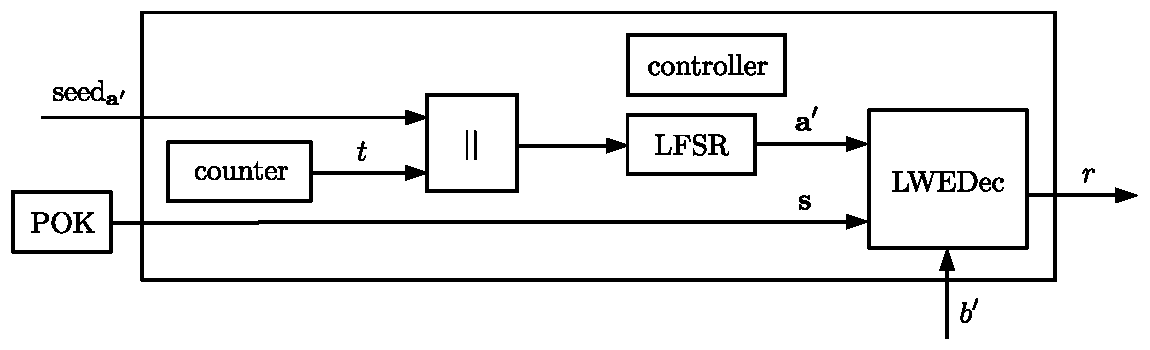
\includegraphics[width = 0.95\linewidth]{./fig/TopLevelDesign.pdf} 
\end{figure}    
\begin{itemize}
    \item Core module: LWE decryption function
    \item Physically obfuscated key (POK) to implement secret $\mathbf{s}$
    \item LFSR-based PRNG to reduce challenge size
    \item Self-incrementing counter to prevent challenge manipulation attack
\end{itemize}
\end{frame}

\begin{frame}{Core Module: LWE Decryption Function}
 \begin{figure}
    \centering
    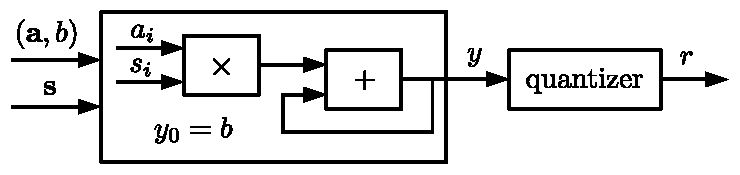
\includegraphics[width = 0.7\linewidth]{./fig/LWEDec.pdf} 
\end{figure}   
\begin{itemize}
    \item Challenge $\mathbf{c}$ mapping to $(\mathbf{a},b)$ via binary vector flattening
\begin{align*}
a_i &= \sum_{j=0}^{\log q-1}c_{(i-1)\log q+j}2^j,\; \forall i\in \{1,2,\ldots,n\}, \\
b &= \sum_{j=0}^{\log q-1}c_{n\log q+j}2^j. 
\end{align*}    
%    \item Modulo operation naturally implemented by fixed-length MAC 
%   \item Quantizer implemented by a integer comparator
\end{itemize}
\end{frame}

\begin{frame}{Parameter Selection in LWE Decryption Function}
\begin{itemize}
\item Major implementation costs: number of challenge and secret bits needed 
    \begin{itemize}
        \item Both scales with $n$ and $\log q$
    \end{itemize}
\item Output errors include environmental errors of secret bits and decryption errors
     \begin{itemize}
        \item POK failure rate needs to be low ($10^{-6}$) since single bit-flip completely changes the CRP behavior of LWEDec
        \item Decryption error due to error terms scales with $m$ and $\alpha$
    \end{itemize}   
\item Concrete ML hardness established by state-of-theart attacks on the LWE cryptosystem scales with $n$ and $\alpha$
%    \begin{itemize}
%        \item Set it to 128bit
%    \end{itemize}
\end{itemize}
\end{frame}

\begin{frame}{Cost vs. Reliability with 128-Bit Concrete Hardness}
\begin{figure}
\centering
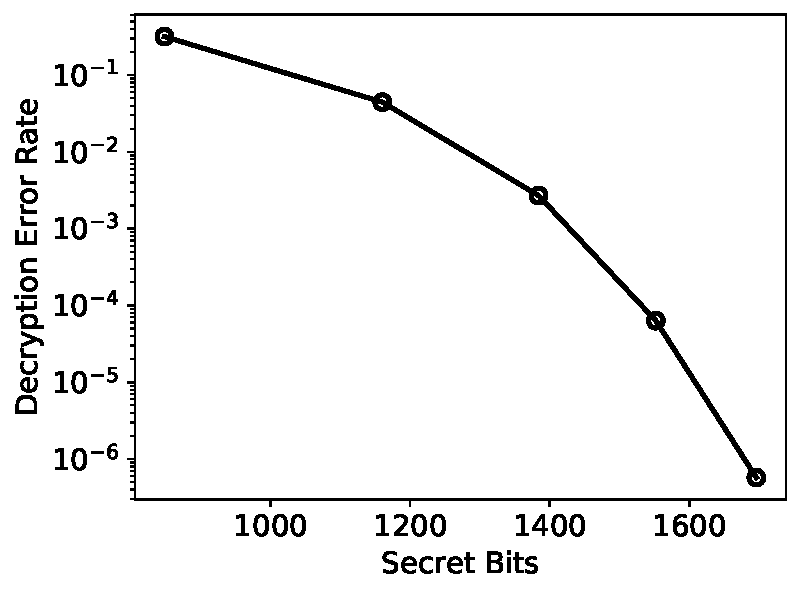
\includegraphics[width=.7\linewidth]{fig/DecErrVsSecretBits.pdf}
\end{figure}   
\begin{itemize}
    \item $n = 160$, $q = 256$, $m = 256$ and $\alpha = 2.20\%$ $\rightarrow$ $128$-bit concrete hardness and decryption error rate of $1.26\%$.
\end{itemize}
\end{frame}

\begin{frame}{Challenge Compression via Distributional Relaxation}
\begin{itemize}
    \item  High ratio (1288:1) of challenge length to response length limits its practical use 
%    \begin{itemize}
%        \item In direct authentication, 100 bits of response requires 128.8K challenge bits transmitted
%    \end{itemize}
    \item Replacing $\mathbf{a}=\mathbf{A}^T\mathbf{x}$ by uniformly sampled $\mathbf{a}^*$ preserves the security properties []
 \begin{equation*}
    \begin{cases}
    \mathbf{a}= \mathbf{A}^T\mathbf{x}\\
    b = (\mathbf{A}^T\mathbf{x})^T\mathbf{s}+\mathbf{e}^T\mathbf{x}+r\floor{q/2}
    \end{cases}\rightarrow\;
    \begin{cases}
    \mathbf{a}^*\\
    b^*=\mathbf{a}^{*T}\mathbf{s}+\mathbf{e}^T\mathbf{x}+r\floor{q/2}
    \end{cases}
\end{equation*}   
\item Space-efficient LWE allows using PRNG to generate $\mathbf{a}^\prime$ with a seed $\text{seed}_{\mathbf{a}^\prime}$ and the corresponding $b^\prime$ becomes
\begin{align*}
    b^\prime&=(\mathbf{a}^\prime)^T\mathbf{s}+\mathbf{e}^T\mathbf{x}+r\floor{q/2}\\
    &= \LFSR{(\text{seed}_{\mathbf{a}^\prime})}^T\mathbf{s}+\mathbf{e}^T\mathbf{x}+r\floor{q/2}.
\end{align*}
    \begin{itemize}
        \item Only need to transmit short seeds
        \item Concrete ML hardness is still preserved
    \end{itemize}
\end{itemize}
\end{frame}

\begin{frame}{Counter Measure for Active Attack}
\begin{itemize}
    \item ML attack belongs to passive attacks
    \item LWE decryption function vulnerable to an active input challenges manipulation attack
    TODO: a figure shows how this attack works
    \item Embed a self-incrementing counter into the challenge seed []
    \begin{itemize}
        \item  restricts the attacker’s ability to completely control input challenges
    \end{itemize}
\end{itemize}
\end{frame}

\begin{frame}{Statistical Properties of Lattice PUF}
   \begin{figure}
  \begin{subfigure}[b]{0.45\textwidth}
    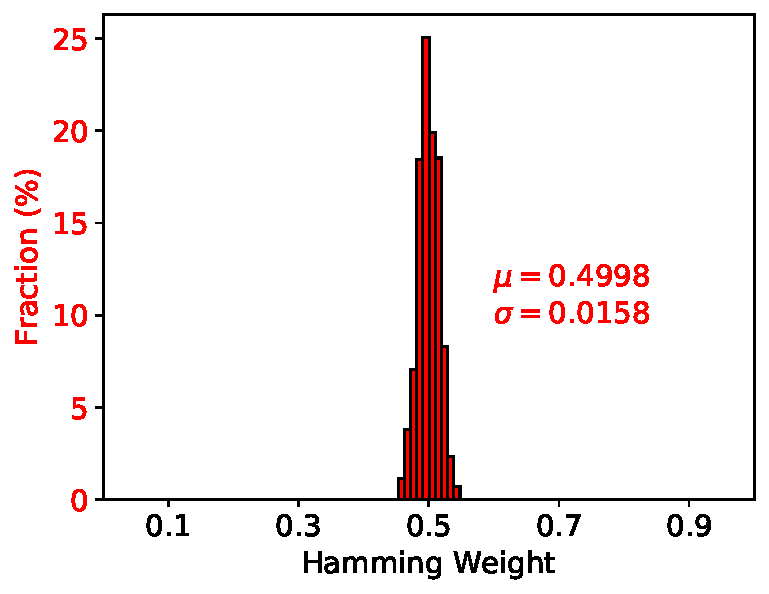
\includegraphics[width=\textwidth]{fig/Uniformity.pdf}
    \caption{Uniformity}
    \label{fig:1}
  \end{subfigure}
  %
  \begin{subfigure}[b]{0.5\textwidth}
    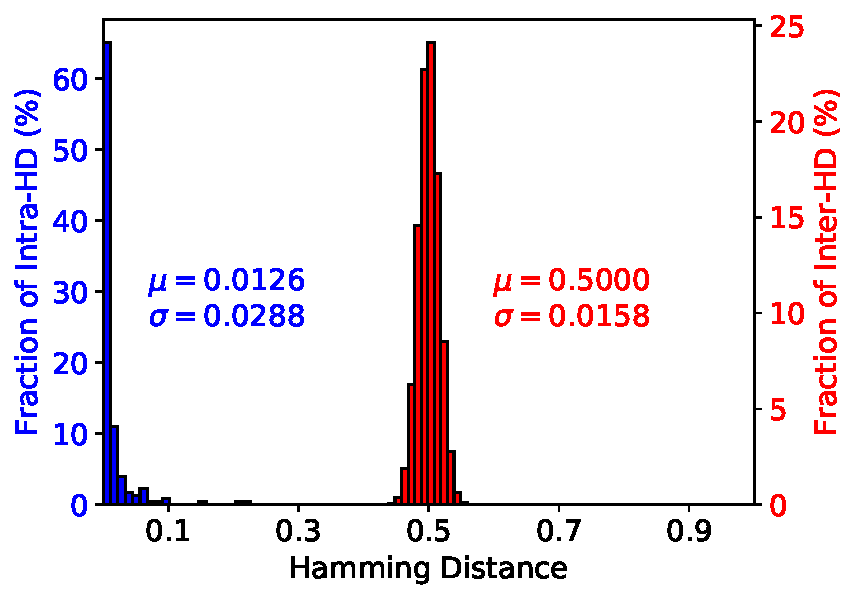
\includegraphics[width=\textwidth]{fig/UniquenessReliability.pdf}
    \caption{Uniqueness and Reliability}
    \label{fig:2}
  \end{subfigure}
\end{figure} 
\begin{itemize}
    \item Evaluated using 1000 randomly instantiated lattice PUFs, each with 1000 randomly generated challenges
\end{itemize}
\end{frame}

\begin{frame}{Empirical ML Resistance}
    \begin{figure}
  \begin{subfigure}[b]{0.48\textwidth}
    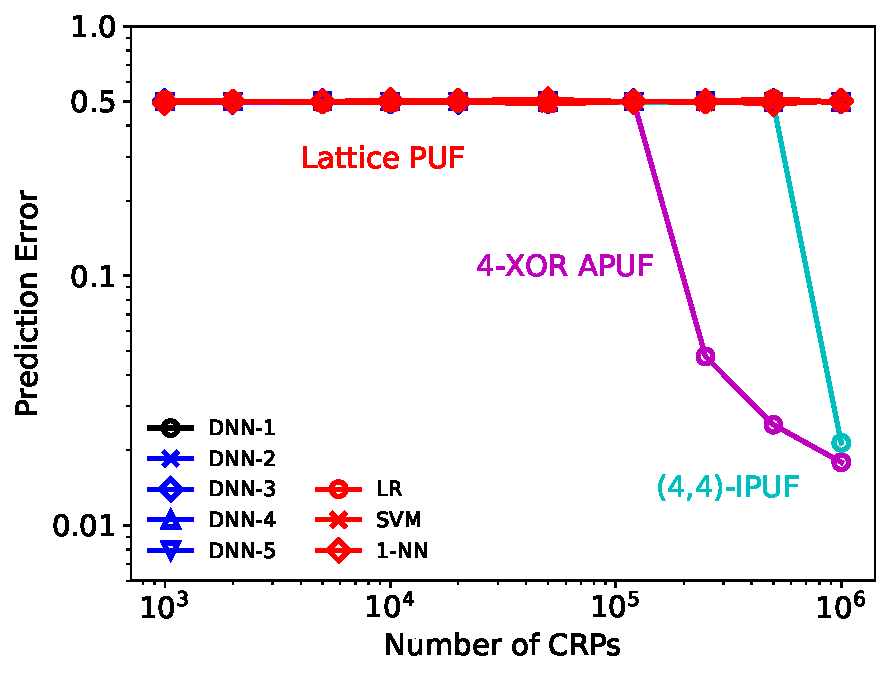
\includegraphics[width=\textwidth]{fig/DNNAllPUFs.pdf}
    %\caption{Uniformity}
    \label{fig:1}
  \end{subfigure}
  %
  \begin{subfigure}[b]{0.48\textwidth}
    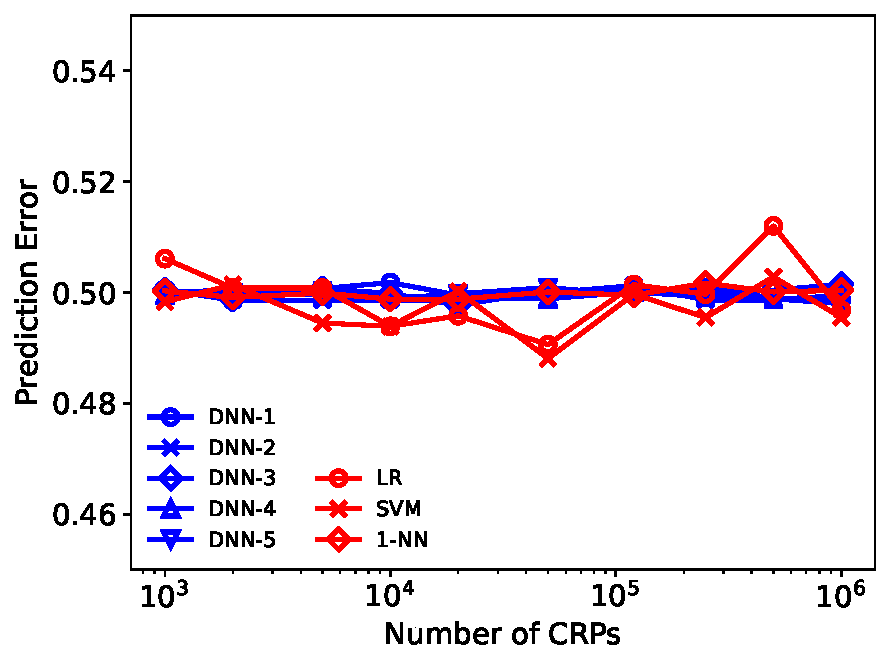
\includegraphics[width=\textwidth]{fig/MLAttackLatticePUF.pdf}
    %\caption{Uniqueness and Reliability}
    \label{fig:2}
  \end{subfigure}
  
\end{figure}   
\begin{table}[t!]
\centering
	%\caption{Various configuration for DNN attacks.}
	\label{table:DNNSetting}
	\resizebox{.6\textwidth}{!}{
\begin{tabular}{|l|l|l|l|l|l|}
\hline
Setup & \begin{tabular}[c]{@{}l@{}}Hidden\\ Layers\end{tabular} & \begin{tabular}[c]{@{}l@{}}Neurons\\ per Layer\end{tabular} & \begin{tabular}[c]{@{}l@{}}Challenge \\ Distribution\end{tabular} & \begin{tabular}[c]{@{}l@{}}Input \\ Format\end{tabular} & \begin{tabular}[c]{@{}l@{}}Prediction\\ Error\end{tabular} \\ \hline
DNN-1     & 4                                                       & 100                                                         & PRNG                                                              & Binary                                                  & 49.86\%                                                       \\ \hline
DNN-2     & 4                                                       & 100                                                         & PRNG                                                              & Real                                                    & 49.84\%                                                       \\ \hline
DNN-3     & 4                                                       & 100                                                         & Ciphertext                                                        & Binary                                                  & 49.76\%                                                       \\ \hline
DNN-4     & 6                                                       & 100                                                         & PRNG                                                              & Binary                                                  & 49.80\%                                                       \\ \hline
DNN-5     & 4                                                       & 200                                                         & PRNG                                                              & Binary                                                  & 49.87\%                                                       \\ \hline
\end{tabular}
}
\end{table}
\end{frame}

\begin{frame}{Hardware Implementation Results}
\begin{itemize}
    \item Entire design, PUF logic and fuzzy extractor (FE), Synthesized, configured, and tested on a Xilinx Spartan-6 FPGA 
    \begin{itemize}
        \item Raw SRAM bits not included
    \end{itemize}
    \item  FE design based on error-correcting codes (ECC): 
\begin{figure}
\centering
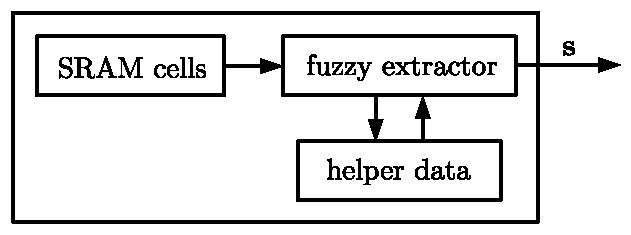
\includegraphics[width=.5\linewidth]{fig/POK.pdf}
\end{figure}    
    \begin{itemize}
        \item Key reconstruction of 1280 bits with
targeted failure rate $10^{-6}$
        \item Concatenation code: repetition code + shortened BCH code
        \item Explore design costs with BER $1\%$, $5\%$, $10\%$, and $15\%$
    \end{itemize}
\end{itemize}
    
\end{frame}

\begin{frame}{Hardware Implementation Results: PUF Logic}
\begin{itemize}
    \item Reference implementation on Spartan-6 FPGA
    \begin{table}[t!]
    %\caption{Reference lattice PUF implementation on Xilinx Spartan-6 FPGA.}
    \label{table:fpga_result}
    \centering
    \def\arraystretch{1.1}
    \subfloat[Area consumption]{
        \resizebox{0.3\linewidth}{!}{
            \begin{tabular}{|c|c|}
            \hline
            \textbf{Module}         & \textbf{Size [slices]} \\ \hline
            LFSR                    & 27            \\ \hline
            LWEDec                  & 2             \\ \hline
            Controller              & 16            \\ \hline
            \textit{Total}          & 45            \\ \hline
            \end{tabular}
            \label{table:fpga_utilization}
        }
    }
    \hspace{1em}
    \subfloat[Runtime]{
        \resizebox{0.5\linewidth}{!}{
            \begin{tabular}{|c|c|}
            \hline
            \textbf{Step}                               & \textbf{Time [$\mu$s]} \\ \hline
            Seed $\text{seed}_{\mathbf{a}'}||t$ load for LFSR    & 8             \\ \hline
            1-bit decryption from LWEDec                  & 44            \\ \hline
            \textit{Total} @ 33 \textit{MHz}            & 52            \\ \hline
            \end{tabular}
            \label{table:fpga_timing}
        }
    }
\end{table}
\item Lightweight compared with other strong PUFs
\begin{table}[t!]
\centering
	%\caption{Hardware implementation costs of strong PUFs.}
	\label{table:hardware_puf}
	\def\arraystretch{1.1}
	\resizebox{0.6\linewidth}{!}{
        \begin{tabular}{|c|c|c|}
        \hline
        \textbf{Design}                                         & \textbf{Platform}  & \textbf{PUF Logic [Slices]} \\ \hline
        POK+AES []                    & Spartan 6 & 80                 \\ \hline
        Controlled PUF []             & Spartan 6 & 127                \\ \hline
        CFE-based PUF []  & Zynq-7000 & 9,825              \\ \hline
        Lattice PUF                                             & Spartan 6 & 45                 \\ \hline
        \end{tabular}
    }
    \vspace{-1em}
\end{table}

\end{itemize}
\end{frame}

\begin{frame}{Hardware Implementation Results: FE}
\begin{itemize}
    \item Configuration of error-correcting codes
    \begin{table}
    \centering
	%\caption{Configuration of error-correcting codes.}
	\vspace{0.5em}
	\label{table:ecc}
	\def\arraystretch{1.1}
	\resizebox{0.65\linewidth}{!}{
        \begin{tabular}{|c|c|c|c|c|c|}
        \hline
        \multirow{2}{*}{\begin{tabular}[c]{@{}c@{}}\textbf{Raw BER}\\  \textbf{(\%)}\end{tabular}} & \multicolumn{2}{c|}{\textbf{Error-Correcting Code}}                                 & \multirow{2}{*}{\textbf{Raw POKs}}  \\ \cline{2-3} 
                                                                                 & Outer code   & Inner code & \\ \hline
        1                                                                        & {[}236, 128, 14{]}  & N/A            & 2,360  \\ \hline
        5                                                                        & {[}218, 128, 11{]} & {[}3, 1, 1{]}  & 6,540  \\ \hline
        10                                                                       & {[}220, 128, 12{]} & {[}5, 1, 2{]}  & 11,000  \\ \hline
        15                                                                       & {[}244, 128, 15{]} & {[}7, 1, 3{]}  & 17,080   \\ \hline
        \end{tabular}
    }
\end{table}

    \item Hardware utilization of FE on Spartan 6 FPGA.
    \begin{table}
    \centering
    %\caption{Hardware utilization in FE design on Spartan 6 FPGA.}
    \label{table:hardware_fe}
	\resizebox{0.8\linewidth}{!}{
        \begin{tabular}{|c|c|c|c|c|c|c|c|c|c|}
        \hline
        \multirow{2}{*}{\begin{tabular}[c]{@{}c@{}}\textbf{Raw BER}\\  \textbf{(\%)}\end{tabular}} & \multicolumn{3}{c|}{\textbf{Outer Code}} & \multicolumn{3}{c|}{\textbf{Inner Code}} & \multicolumn{3}{c|}{\textbf{Total}} \\ \cline{2-10} 
                               & Reg      & LUT      & Slice     & Reg      & LUT      & Slice     & Reg    & LUT    & Slice    \\ \hline
        1                      & 905      & 893      & 276       & 0        & 0        & 0         & 905    & 893    & 276      \\ \hline
        5                      & 730      & 688      & 232       & 0        & 1        & 1         & 730    & 689    & 233      \\ \hline
        10                     & 785      & 740      & 243       & 0        & 3        & 2         & 785    & 743    & 245      \\ \hline
        15                     & 973      & 913      & 326       & 0        & 7        & 3         & 973    & 920    & 329      \\ \hline
        \end{tabular}
    }
\end{table}
\end{itemize}
\end{frame}

\begin{frame}{Conclusions}
\begin{itemize}
    \item  A strong PUF provably secure against machine learning (ML) attacks
    \begin{itemize}
        \item Security derived from hardness assumptions on lattice problems
        \item Exhibit empirical ML resistance even with advanced DNN attacks
    \end{itemize}
    \item Excellent uniformity, uniqueness, and reliability.
    \item Lightweight hardware implementation via distributional relaxation
\end{itemize}    
\end{frame}